\chapter{Représentation du réseau routier}
Un graphe sert mieux à définir l'existence d'une relation entre objets tels qu'une ligne entre deux stations de métro, ce qui est la représentation optimale pour nos données. Dans ce chapitre, nous présenterons en première partie les définitions relatives aux graphes et recherche de chemins, ensuite nous discuterons les différentes approches de représentation prises en compte et les spécifications de nos données, enfin nous détaillerons la représentation choisie en donnant des exemples.

\section{Généralités sur les graphes}
La théorie des graphes est très probablement née en 1735 lorsque Leonhard Euler (1707 - 1783) résout le problème des sept ponts de Königsberg. 
L'énoncé de ce problème est: la ville de \emph{Königsberg} est une ville autour d'un fleuve, elle compte quatre berges et sept ponts les reliant. Le but du jeu est de savoir s'il existe un chemin permettant d'emprunter tous les ponts une fois et une seule et revenir au point de départ. Le problème s'appelle désormais, de façon plus formelle, la recherche d'un cycle eulérien dans un graphe. Euler a démontré que ce problème n'avait pas de solution.

\begin{figure}[h!]
\center
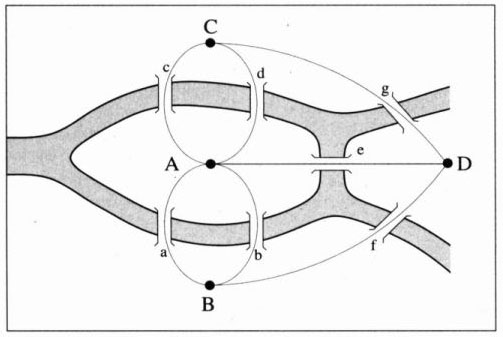
\includegraphics[width=0.75\textwidth]{img/Bridges.jpg}
\caption{Démonstration du problème des septs ponts de Königsberg}
\end{figure}

\subsection{Définitions}
\begin{description}
\item[Graphe]: un graphe est composé de sommets (\textbf{vertices}) ou noeuds (\textbf{nodes}), et d'arcs (\textbf{edges}) ou d'arêtes (\textbf{links}) reliant certains de ces sommets ou noeuds.
Un graphe G est défini de manière formelle par un couple (S,A) où :
\begin{itemize}
	\item S est un ensemble fini d'éléments. Chacun de ces éléments est appelé sommet du graphe.
	\item A est un sous-ensemble (éventuellement nul) de SxS. Chacun de ces éléments de A est appelé arc ou arête.
\end{itemize}
Chaque arc est associé à un poids ou une étiquette qui le décrit. Par exemple, dans un réseau social il peut définir la nature de la relation (ami, famille, collègue) et dans un réseau routier la longueur d'une rue. Parfois le terme coût est utilisé.

\item[Graphe connexe] : un graphe est connexe si on peut atteindre n'importe quel sommet à partir d'un sommet quelconque en parcourant différentes arêtes.

\item[Graphe directionnel] : aussi appelé graphe orienté, digraphe ou un réseau dirigé, c'est un graphe où les sommets (nœuds) sont connectés ensemble, et tous les bords sont dirigés d'un sommet à l'autre. Les bords sont généralement des flèches dessinées indiquant la direction.
Un graphe où les bords sont bidirectionnels est appelé un graphique non orienté.

\item[Chemin] : un chemin est une séquence finie et alternée de sommets et d'arcs, débutant et finissant par des sommets, tel que chaque arc sortant d'un sommet est incident au sommet suivant dans la séquence (cela correspond à la notion de chaîne \emph{orientée}).
\begin{figure}[h]
	\centering
	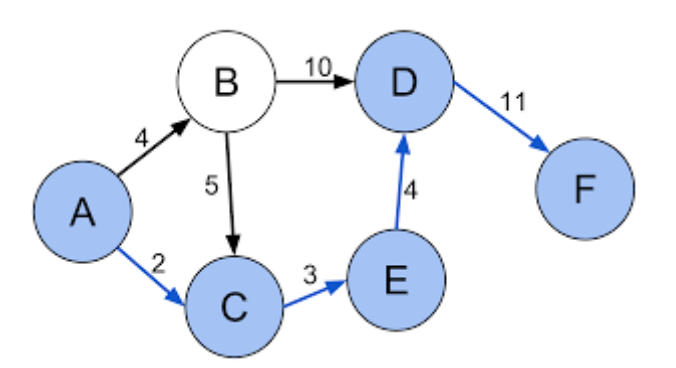
\includegraphics[width=0.75\textwidth]{img/cheminGraphe.png}
	\caption{Exemple de chemin orienté}
\end{figure}
\end{description}

	
	
\section{Avantages d'utilisation d'un graphe}
\subsection{Domaines d'utilisation des graphes}
Un graphe sert avant tout à manipuler des concepts, et à établir un lien entre ces concepts. N'importe quel problème comportant des objets avec des relations entre ces objets peut être modélisé par un graphe.
Les graphes sont donc des outils très puissants et largement répandus qui se prêtent bien à la résolution de nombreux problèmes. Voici quelques-uns :

\subsection{Recherche de chemin (PathFinding)}
Un cas très fréquent. Chaque nœud représente une position et chaque arête est un chemin entre deux positions, ou en remplaçant les nœuds par des adresses et les arêtes par des routes, on obtient le graphe utilisé par les GPS ou Google Map par exemple.
La recherche de chemins est aussi utilisée en biologique, communications (réseaux de télécommunications), réseau hydrographique...etc.
Il est courant de chercher le chemin le plus court entre deux positions dans la plupart de ces domaines, nous nous intéressons particulièrement à ce cas d'utilisation, que nous discutons en détail dans la section suivante.


\subsection{L'ordonnancement de tâches:}
On peut représenter chacune des tâches à effectuer par un nœud, et les dépendances entre chacune de ces tâches par des arêtes.
On cite l'exemple de l'ordonnancement des projets, les graphes permettent de planifier les différentes tâches d'un projet, détecter les tâches pouvant être effectuées simultanément et estimer la durée totale du projet.

\subsection{Les systèmes de recommandation:}
C'est une forme spécifique de filtrage de l'information qui a pour but de présenter à un utilisateur des éléments qui sont susceptibles de l'intéresser, en se basant sur ses préférences et son comportement.
Les moteurs de recommandation font usage des graphes pour représenter des individus ou objets et leurs différents liens. Cet outil est très utilisé en sciences sociales, par exemple le graphe social de Facebook qui représente les associations entre des personnes ou le réseau LinkedIn qui est un graphe de relations entre des professionnels...etc.

Le but est de pouvoir identifier les communautés formées, les centres d'intérêts communs, en suggérant à l'utilisateur les choses qu'il est susceptible d'aimer, les personnes qu'il connaît peut-être, et avant tout (et surtout) pour créer des publicités ciblées adaptées à chacun.


\section{Recherche de Chemin:}

\subsection{Définition:}
La recherche du plus court chemin est la capacité pour un système de déduire le chemin approprié autour des obstacles pour atteindre un point de destination tout en évitant les obstacles et en parcourant la distance la plus petite possible.
Le choix de la méthode de l'analyse et sa complexité peuvent augmenter à mesure que d'autres circonstances doivent être analysées, en prenant en compte différentes contraintes :

\begin{itemize}
	\item \textbf{Poids:} certains algorithmes n'acceptent que des arcs dont le poids est positif.
	\item \textbf{Chemins calculés:} il existe des algorithmes qui calculent le plus court chemin de nœud à nœud, entre toutes les paires de nœuds ou encore d'un nœud vers tous les autres.
	\item \textbf{Prise en compte d'informations externes:} l'utilisation d'une connaissance externe à la structure du graphe peut parfois accélérer la recherche.
\end{itemize}

\subsection{Domaines d'utilisation :}
Le problème du plus court chemin est parmi les problèmes les plus étudiés de la théorie des graphes, on le retrouve dans beaucoup de domaines :
\begin{itemize}
\item\textbf{Economie:} problèmes d’investissement
\item\textbf{Gestion:} gestion des projets
\item\textbf{Optimisation des réseaux:} réseaux routiers, de télécommunications, de distribution.
\item\textbf{Réseaux informatiques et protocoles de routage:}   protocole OSPF: Open Shortest Path First.
\item\textbf{Biologie:} il est utilisé pour trouver le modèle de réseau dans la propagation d'une maladie infectieuse, par exemple.
\item\textbf{Cartographie:} pour mesurer le chemin le plus court entre deux lieux ou villes.
\item\textbf{Jeux vidéo}.
\item\textbf{robotique}.
\end{itemize}

\subsection{Les algorithmes de recherche de chemin}
(Reste à détailler brievement les differents algorithmes) \newline
Les algorithmes de calcul d'itinéraires origine-destination(s) sont de complexité polynomiale et on les répartit classiquement en deux familles : ceux à fixation d'étiquettes (algorithme de Dijkstra) et ceux à correction d'étiquettes (algorithme de Bellman-Ford).
Malgré leur complexité polynomiale, ces algorithmes peuvent néanmoins engendrer des temps de calculs importants pour des graphes de grande taille, ce qui a suscité le développement des techniques d'accélération (visant souvent l'optimalité) comme l'algorithme A*, le parcours bidirectionnel, ainsi que les méthodes de pré-traitement.
\newline

** Parler de A* et son éfficacité, puis expliquer pourquoi on l'utilise pas ( à mettre dans les perspectives ) à cause de la fonction d'heuristique qui est difficile à concevoir sans une bonne connaissance de ce probleme (dans les limites du temps du projet), considerer donc une approche plus simple utilisant l'algorithme BFS qui est facile à mettre en oeuvre et à "customiser" à nos besoins.

\subsection{L'algorithme BFS (Breadth-First-Search)}
\begin{itemize}
\item présenter l'algorithme
\item Parler de complexité et pourquoi avoir choisi
\item Code/algorithme de .. l'algorithme.
\end{itemize}

\section{Données collectées}
Afin de mieux tester notre application, nous avons tenté de collecter un maximum de données réelles, à commencer par contacter l'Entreprise de Transport d'Oran, puis ensuite traiter ces informations et ajouter d'autres que nous avons collectés par nous-mêmes.
Le résultat de cette collecte est comme suit :

\subsection{ETO (Entreprise de Transport d'Oran)}

%what they did gave u
Nous avons été bien accueillis par l'un des responsables de l'ETO que nous remercions de nous avoir bien expliqué le fonctionnement des lignes de notre région ainsi que d'avoir fourni plusieurs informations utiles, tel que:
\begin{itemize}
	\item La liste des lignes et leur longueur totale.
	\item Les différents horaires de travail (été/hiver/fin de semaine...etc).
	\item La fréquence des bus et les différentes contraintes spécifiques à notre région.
	\item Le nombre de bus desservant chaque ligne .
	\item Le nom de chaque station.
\end{itemize}

% but that wasnt enough
En plus du catalogue que nous avons reçu, leurs informations nous ont permis de bien tracer les spécifications et les particularités de ces lignes.
Cependant, ces informations n'ont pas été suffisantes pour notre travail, en effet:
	\begin{itemize}
	\item Nous avions besoin de noms plus significatifs pour chaque station, car les noms fournis étaient des noms communs connues par les habitants seulement.
	\item Le catalogue ne contenant pas les adresses exacte ou les coordonnées de chaque station.
	\item Pas d'informations sur la distance entre chaque station.
	\end{itemize}
	
%thx again for trying
Nous remercions encore l'ETO pour leur assistance, néanmoins ces données doivent être traitées d'avantage, réorganisées et complétées avant qu'elles puissent être intégrées dans notre application.

** Aperçu du deuxieme tableau global reçu pour la frequence et lignes.

\subsection{Traitement de données}

** Image du avant et après

\begin{itemize}
	\item **Par manque de données, nous ne pouvons pas importer directement ces lignes vers l'application, d'où nécessite d'implémenter une Interface pour mieux introduire les lignes et stations, aperçu du résultat dans la section \ref{ref:Implementation} du chapitre 4.
\end{itemize}

\subsection{Données supplémentaire}
	\begin{itemize}
		\item Parler des données de Tramway récupérées depuis le site de Setram.
		\item Parler de l'idée du crowd-sourcing
	\end{itemize}
	
\section{Construction du graphe}
\subsection{Différentes approches pour stocker le graphe}
\begin{itemize}
	\item \textbf{Outils Open Source (OpenTripPlanner} : 
	      Il existe plusieurs outils qui proposent ce service, en particulier OpenTripPlanner : un projet Open Source qui permet de créer un réseau routier à partir de données GTFS \FancyFootNote{GTFS (General Transit Feed Specification : ...}, ces données seront ensuite intégrées avec OpenStreetMap et stockées sur le serveur, qui exposera une API REST pour questionner le serveur : recherche de Chemin, possibilité d'intégrer les horaires, ...etc.
	      		
	      Vu la nature un peu particulière du réseau d'Oran, et la non-disponibilité des données (Données officielles des lignes et données (adresses) sur OpenStreetMap), cette solution ne sera pas envisagée. 
	      Cependant, l'application prendra une architecture flexible permettant d'intégrer, au futur, de tels outils rapidement au cas de nécessité.
	\item \textbf{Représentation indépendante de chaque ligne}
	      Une des approches considérées était de représenter chaque ligne indépendamment, l'algorithme du service aura à chercher des points de liaison entre ces lignes.
	      L'avantage principal de cette approche est la facilité de manipulation de ces données de lignes, en ajoutant/supprimant des lignes sans conflit.
	      Cette approche présente par contre un inconvénient majeur au niveau de performance, vu que l'utilisation d'un algorithme de PathFinding requiert l'utilisation de plusieurs tables (lignes) à chaque requête. Ce qui nous a menés à l'approche suivante.
	\item \textbf{Représentation en graphe (Base de données orientée graphe}: nous avons finalement opté vers une représentation en graphe, qui est la plus intuitive dans notre cas, et qui permet aussi un accès plus rapide et simple en parcourant un graphe déjà construit, tout en tirant les meilleures performances des différents algorithmes de recherche de chemins.
	On utilisera pour cela une base de données orientée graphe, qui permet de stocker en permanence le graphe, mais aussi de fournir plusieurs opérations pour créer, modifier et parcourir nos graphes.
	
	Nous a, cependant, noté certaines difficultés suivant cette représentation, notamment dans la modification ou suppression de lignes où le changement ou suppression d'une seule station peut affecter plusieurs autres lignes ou par example l'ajout d'une station au milieu d'une ligne impliquera la suppression de plusieurs arcs.
	Comme première solution, nous avons décidés de restreindre les modifications et suppressions de nœuds aux stations qui ne sont reliées à aucune ligne, et pour les lignes, de supprimer toute la ligne et reconstruire les arcs à chaque modification.
	     
\end{itemize}
\subsection{Représentation choisie du graphe}
	\begin{itemize}
	\item Présenter en détail la représentation
	\item Donner la structure du graphe ( trouver une façon pour représenter proprement ces informations : )
	\begin{itemize}
		 \item  neouds représentent station
		 \item Arcs representent un tronçon/chemin entre deux stations
		 \item Arcs étiquetés par le type du transport ( BusSegment, TramSegment, WalkSegment. ..) 
		 \item Représenter chaque bus séparément ( pour faciliter la recherche et filtre ) 
		 \item Nœuds (Stations) ont les attributs suivants : 
		 \begin{itemize}
		 	\item Nom.
		 	\item Adresse.
		 	\item Tableau de coordonnées (pour chaque direction) avec indicateur de direction.
		 \end{itemize}
		 \item Arcs ont les attributs suivants :
		 \begin{itemize}
		 		\item Dist : distance entre les deux stations
		 		\item Time: temps moyen pour passer de la première station à la deuxieme
		 		\item Bus : ( pour les arcs de type Bus ) nom/id du bus.
		 		** remarque : infos du bus ( temps d'arrêt, prix ..etc) sont stockés sépareraient.
		 \end{itemize}
	\end{itemize}
	\end{itemize}

\subsection{Résultat final}
	** Capture d'écran d'un graphe exemple.

\subsection{Conclusion}

** Malgré les différentes contraintes (données manquantes, horaires non régulières...etc.), la représentation choisie reste suffisante et facilement extensible pour de futures améliorations.
\newpage
